\section{Traceroute a Universidades}

A continuación mostramos diferentes traceroutes a universidades en diferentes continentes. Consideramos que esto es relevante dado que nos permitirá observar enlaces intercontinentales y otras particularidaades. El RTT promedio se calculo a partir de 5 requests. El host name lo conseguimos a partir de la funcion socket.gethostbyaddr de Python, que lo que hace es simplemente un DNS lookup \footnote{El manpage de la libc explica como se hace esto \url{http://www.freebsd.org/cgi/man.cgi?query=gethostbyaddr&sektion=3&manpath=FreeBSD+6.0-RELEASE}}. La ubicación la conseguimos a partir de una base de datos publica de GeoIP.

\subsection{dc.ubar.ar}

\begin{table}[H]
\centering
\caption{traceroute: dc.uba.ar}
\begin{tabular}{@{}lllll@{}}
\toprule
Hop & Avg. RTT & IP Address & Host name & Location\\ \midrule
1 & 9.3842 ms & 181.169.12.1 & 1-12-169-181.fibertel.com.ar & AR, SA\\
2 &  * * * * * &  &  &  \\
3 &  * * * * * &  &  &  \\
4 &  * * * * * &  &  &  \\
5 & 14.025 ms & 200.89.164.53 & 53-164-89-200.fibertel.com.ar & AR, SA\\
6 & 14.7514 ms & 200.89.165.2  & 2-165-89-200.fibertel.com.ar & AR, SA\\
7 & 22.5916 ms & 200.89.165.86 & 86-165-89-200.fibertel.com.ar & AR, SA\\
8 & 16.5408 ms & 200.49.69.161 & VPN-corp.metrored.net.ar & AR, SA\\
9 &  * * * * * &  &  &  \\
10 &  * * * * * &  &  &  \\
11 &  * * * * * &  &  &  \\
12 & 12.7052 ms & 157.92.47.53 & 157.92.47.53 & AR, SA\\
13 & 13.067 ms & 192.168.121.2 & 192.168.121.2 &  \\
14 &  * * * * * &  &  &  \\
... &  * * * * * &  &  &  \\

 \bottomrule
\end{tabular}
\label{dc}
\end{table}

Como es de esperar, al hacer un request a dc.uba.ar desde Argentina no hay saltos intercontinentales. Sin embargo, notemos que este traceroute cae en el problema de missing destination. Esto no es porque el servidor no exista, si no porque probablemente esta configurado para no devolver ICMP requests.

Intentamos acceder a metrored.net.ar, ya sea por URL o por IP y no lo logramos. Sin embargo, al hacer un IP Whois encontramos:

\begin{table}[H]
\centering
\caption{Whois lookup: metrored.net.ar}
\begin{tabular}{@{}ll@{}}
\toprule
owner:       &   Techtel LMDS Comunicaciones Interactivas S.A. \\
ownerid:     &   AR-TLCI-LACNIC \\
responsible: & Administrador de Direcciones IP - CLARO \\
address:     &   Garay, 34 \\
address:     &   C1063AB - Buenos Aires \\
country:     &   AR \\
phone:       &   +54 11 4000-3000 [3270] \\
nserver:     &   DNSMR1.METRORED.NET.AR   \\ \bottomrule
\end{tabular}
\end{table}

Por lo que podemos ver, el hop pertenece a Claro.

\subsection{mit.edu}

\begin{table}[H]
\caption{traceroute: mit.edu}
\centering
\begin{tabular}{@{}lllll@{}}
\toprule
Hop & Avg. RTT & IP Address & Host name & Location\\ \midrule
1 & 15.0554 ms & 181.169.12.1 & 1-12-169-181.fibertel.com.ar & AR, SA\\
2 &  * * * * * &  &  &  \\
3 &  * * * * * &  &  &  \\
4 &  * * * * * &  &  &  \\
5 & 15.8334 ms & 200.89.160.13 & 13-160-89-200.fibertel.com.ar & AR, SA\\
6 & 16.5964 ms & 200.89.165.129 & 129-165-89-200.fibertel.com.ar & AR, SA\\
7 & 12.4244 ms & 200.89.165.150 & 150-165-89-200.fibertel.com.ar & AR, SA\\
8 & 11.7036 ms & 195.22.220.154 & xe-1-2-0.baires3.bai.seabone.net & IT, EU\\
9 & 241.317 ms & 89.221.43.117 & xe-5-3-0.londra32.lon.seabone.net & IT, EU\\
10 & 251.369 ms & 149.3.183.55 & 149.3.183.55 & IT, EU\\
11 & 345.3244 ms & 104.65.21.108 & a104-65-21-108.deploy.static.akamaitechnologies.com & NL, EU\\
 \bottomrule
\end{tabular}
\label{mit}
\end{table}

En este gráfico hay un enlace transatlántico claramente identificable entre el hop 7 y el hop 8. Notar que el host name ya indica que es transatlántico. Buscando a quien pertenece seabone.net, averiguamos que pertenece a la empresa Sparkle que provee servicios de enlaces transatlánticos.

\begin{tcolorbox}
Sparkle is a leading global telecommunication service provider, offering a complete range of IP, Data, Cloud, Data Center, Mobile and Voice solutions designed to meet the ever changing needs of Fixed and Mobile Operators, ISPs, OTTs, Media \& Content Players, Application Service Providers and Multinational Corporations (MNCs)
\end{tcolorbox}

\begin{figure}[H]
\caption{RTTs de los hosts hasta mit.edu}
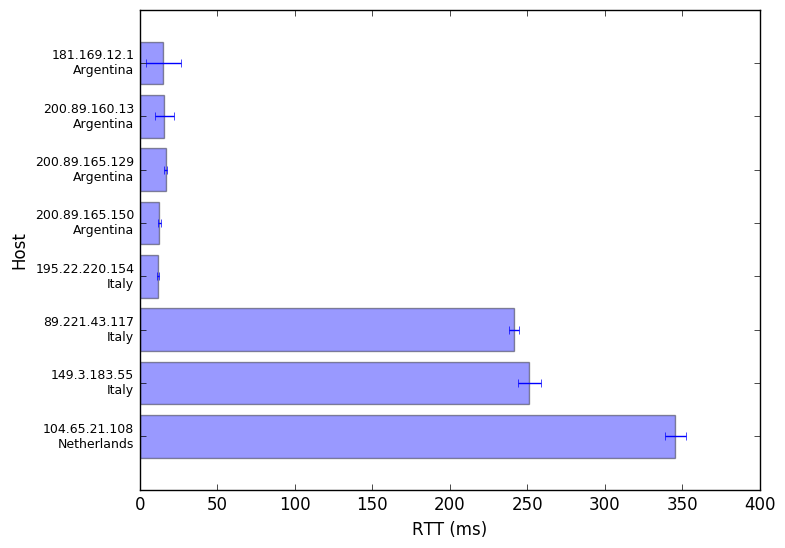
\includegraphics[width=\textwidth,keepaspectratio]{images/mit.png}
\end{figure}

Curiosamente, al final el request termino en Holanda en nodo de Akamai y no en Estados Unidos. Haciendo un Whois al URL confirmamos que esto es correcto.

\pagebreak

\subsection{ox.ac.uk}

\begin{table}[H]
\caption{traceroute: ox.ac.uk (oxford)}
\centering
\begin{tabular}{@{}lllll@{}}
\toprule
Hop & Avg. RTT & IP Address & Host name & Location\\ \midrule
1 & 11.3802 ms & 181.169.12.1 & 1-12-169-181.fibertel.com.ar & AR, SA\\
2 &  * * * * * &  &  &  \\
3 &  * * * * * &  &  &  \\
4 &  * * * * * &  &  &  \\
5 & 19.6882 ms & 200.89.160.13 & 13-160-89-200.fibertel.com.ar & AR, SA\\
6 & 12.336 ms & 200.89.165.250 & 250-165-89-200.fibertel.com.ar & AR, SA\\
7 & 10.678 ms & 190.216.88.33 & 190.216.88.33 & AR, SA\\
8 & 138.477 ms & 67.17.99.233 & ae0-300G.ar5.MIA1.gblx.net & US, NA\\
9 &  * * * * * &  &  &  \\
10 &  * * * * * &  &  &  \\
11 & 230.1234 ms & 212.187.139.166 & unknown.Level3.net & GB, EU\\
12 & 278.9116 ms & 146.97.33.2 & ae29.londpg-sbr2.ja.net & GB, EU\\
13 & 280.8712 ms & 146.97.37.194 & ae19.readdy-rbr1.ja.net & GB, EU\\
14 & 225.575 ms & 193.63.108.94 & ae2.oxfoii-rbr1.ja.net & GB, EU\\
15 & 225.931 ms & 193.63.108.98 & ae3.oxforq-rbr1.ja.net & GB, EU\\
16 & 227.0804 ms & 193.63.109.90 & 193.63.109.90 & GB, EU\\
17 &  * * * * * &  &  &  \\
18 &  * * * * * &  &  &  \\
19 & 282.648 ms & 192.76.32.62 & boucs-lompi1.sdc.ox.ac.uk & GB, EU\\
20 & 275.7754 ms & 129.67.242.154 & aurochs-web-154.nsms.ox.ac.uk & GB, EU\\ \bottomrule
\end{tabular}
\label{oxford}
\end{table}

Aquí podemos identificar claramente enlaces transatlánticos a partir del host name y la ubicación. Level3 es una empresa conocida proveedora de enlaces. Un dato de color, sus acciones cotizan en Nasdaq.

\begin{figure}[H]
\caption{RTTs de los hosts hasta ox.ac.uk}
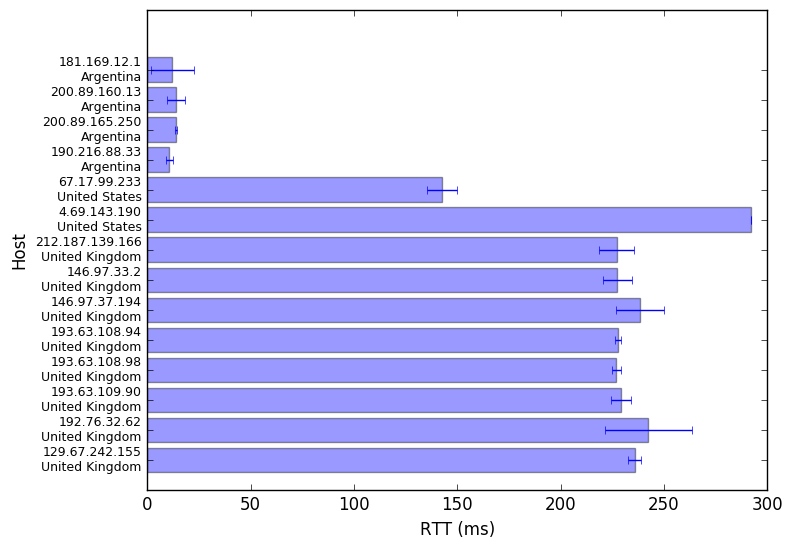
\includegraphics[width=\textwidth,keepaspectratio]{images/oxford.png}
\end{figure}

\subsection{u-tokyo.ac.jp}

\begin{table}[H]
\caption{traceroute: u-tokyo.ac.jp}
\centering
\begin{tabular}{@{}lllll@{}}
\toprule
Hop & Avg. RTT & IP Address & Host name & Location\\ \midrule
1 & 9.9508 ms & 181.169.12.1 & 1-12-169-181.fibertel.com.ar & AR, SA\\
2 &  * * * * * &  &  &  \\
3 &  * * * * * &  &  &  \\
4 &  * * * * * &  &  &  \\
5 & 16.979 ms & 200.89.160.21 & 21-160-89-200.fibertel.com.ar & AR, SA\\
6 & 15.2796 ms & 200.89.165.222 & 222-165-89-200.fibertel.com.ar & AR, SA\\
7 & 10.541 ms & 195.22.220.102 & xe-1-0-3.baires5.bai.seabone.net & IT, EU\\
8 & 39.8348 ms & 195.22.219.17 & ae7.sanpaolo8.spa.seabone.net & IT, EU\\
9 & 36.1798 ms & 195.22.219.17 & ae7.sanpaolo8.spa.seabone.net & IT, EU\\
10 & 42.7854 ms & 149.3.181.65 & 149.3.181.65 & IT, EU\\
11 & 159.2136 ms & 129.250.2.227 & ae-4.r24.nycmny01.us.bb.gin.ntt.net & US, NA\\
12 & 237.3446 ms & 129.250.4.13 & ae-2.r20.sttlwa01.us.bb.gin.ntt.net & US, NA\\
13 & 225.4494 ms & 129.250.2.54 & ae-0.r21.sttlwa01.us.bb.gin.ntt.net & US, NA\\
14 & 426.808 ms & 129.250.3.86 & ae-2.r20.osakjp02.jp.bb.gin.ntt.net & US, NA\\
15 & 429.0596 ms & 129.250.6.188 & ae-4.r22.osakjp02.jp.bb.gin.ntt.net & US, NA\\
16 & 421.2708 ms & 129.250.2.255 & ae-1.r01.osakjp02.jp.bb.gin.ntt.net & US, NA\\
17 & 417.919 ms & 61.200.80.218 & xe-0-4-0-7.r01.osakjp02.jp.ce.gin.ntt.net & JP, AS\\
18 & 425.9262 ms & 158.205.192.173 & ae0.ostcr01.idc.jp & JP, AS\\
19 & 426.6464 ms & 158.205.192.86 & 158.205.192.86 & JP, AS\\
20 & 534.723 ms & 158.205.121.250 & po2.l321.fk1.eg.idc.jp & JP, AS\\
21 & 436.512 ms & 154.34.240.254 & 154.34.240.254 & JP, AS\\
22 & 424.7352 ms & 210.152.135.178 & 210.152.135.178 & JP, AS\\
 \bottomrule
\end{tabular}
\label{tokyo}
\end{table}

\vspace{10px}

Como era de esperar, este termino siendo el traceroute mas largo, pasando por un camino sumamente raro. De Argentina a Italia, luego a EE.UU. y finalmente a Japón. Sin embargo, si vemos esto desde un punto de vista económico tiene sentido. El trafico desde América Latina a Japon no debe ser muy alto, por lo que no se justifican los altos costos de hacer un enlace mas directo.

Encontramos nuevamente los enlaces transatlánticos de Sparkle. Entrando a ntt.net nos encontramos con:

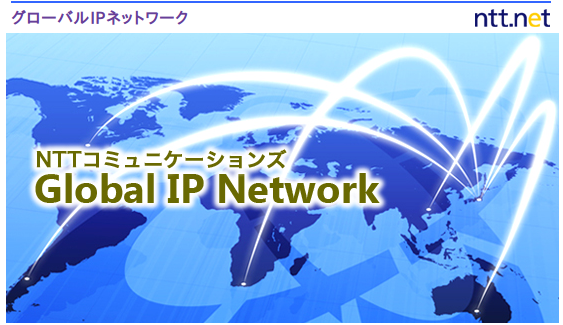
\includegraphics[width=\textwidth,keepaspectratio]{images/ntt}

Esto nos hace inferir que es una empresa Japonesa de telecomunicaciones.